\documentclass{article}
\usepackage[utf8]{inputenc}

\title{Interacting Particle System Thesis}
\author{Stefan Eng}
\date{2019/2020}

\usepackage{amsthm}
\usepackage{amssymb}
\usepackage{amsmath}
\usepackage{hyperref}
\usepackage{caption}
\usepackage{mathrsfs}
\usepackage{blkarray}

\usepackage{natbib}
\usepackage{graphicx}

\usepackage{tikz}
\usetikzlibrary{calc, automata, chains, arrows.meta}


\theoremstyle{plain}
\newtheorem{theorem}{Theorem}[section]
\newtheorem{example}{Example}[section]
\newtheorem{lemma}{Lemma}[section]
\newtheorem{prop}{Proposition}[section]

\theoremstyle{definition}
\newtheorem{defn}{Definition}[section]
\newtheorem{exercise}{Exercise}[section]

\theoremstyle{remark}
\newtheorem*{note}{Note}
\newtheorem*{remark}{Remark}

\newcommand{\R}{\mathbb{R}}
\newcommand{\Rs}{\mathcal{R}}
\newcommand{\Gs}{\mathcal{G}}
\newcommand{\Cs}{\mathcal{C}}
\newcommand{\Q}{\mathbb{Q}}
\newcommand{\A}{\mathcal{A}}
\newcommand{\F}{\mathcal{F}}
\newcommand{\E}{\mathcal{E}}
\newcommand{\M}{\mathcal{M}}
\newcommand{\N}{\mathcal{N}}
\newcommand{\Z}{\mathbb{Z}}
\newcommand{\Zs}{{\{0,1\}^\mathbb{Z}}}
\newcommand{\I}{\mathcal{I}}
\newcommand{\D}{\mathcal{D}}
\newcommand{\B}{{\mathcal{B}_{\mathbb{R}}}}
\newcommand{\BU}{{\mathcal{B}_{[0,1]}}}
\newcommand{\loc}{L_{\text{loc}}^1}
\newcommand{\powset}{\mathcal{P}}
\newcommand{\outm}{\mu^{*}}
\newcommand{\cdict}{\Rightarrow\!\Leftarrow}
\newcommand{\Var}{\operatorname {Var}}

% X_1, ..., X_n
\newcommand{\Xn}{\ensuremath{X_1,\ldots,X_n}}
\newcommand{\xn}{\ensuremath{x_1,\ldots,x_n}}

\begin{document}

\maketitle

\section{Introduction}

\section{Interacting Particle Systems}

\subsection{Contact Process on Finite Graphs}

Now we look at a contact process on a finite graph.
Based on finite Markov chain theory, no matter the initial state, the process will eventually be zero.
We look at $T_\lambda$, the time until we reach the state zero while keeping the number of nodes fixed as $\lambda$ goes to $\infty$.
First we investigate the behavior for a complete graph, in which each node is connected to all other nodes and then we look at the one-dimensional lattice, in which each node is connected to at most two neighbors.

\subsection{Two node contact process}

Define a contact process on the finite graph with two nodes and one edge between them.

\begin{figure}
    \centering
   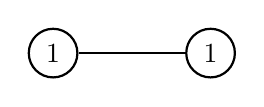
\begin{tikzpicture}[auto, node distance=2cm, every loop/.style={}, thick,main node/.style={circle,draw}]
   \node[main node]  (0) {1};
   \node[main node]  (1) [left of=0]  {1};
   
   \draw (0) edge [left] (1);
\end{tikzpicture}
    \caption{Two node contact process starting with both as ones.}
    \label{fig:two_node_contact}
\end{figure}

\begin{align}
    1 &\to 0 \text{ at rate } 1\\
    0 &\to 1 \text{ at rate } \begin{cases}
        \lambda & \text{ if neighbor is 1}\\
        0 & \text{ otherwise}
    \end{cases}
\end{align}

Start the process with both nodes at 1.
Clearly we will eventually reach $(0,0)$.
We can express the $G$ matrix as

% Info on blockarray
% https://tex.stackexchange.com/a/59519/41827
$$
G = \begin{blockarray}{ccccc}
    & (1,1) & (1,0) & (0,1) & (0,0)\\
    \begin{block}{c(cccc)}
        (1,1) & -2 & 1 & 1 & 0\\
        (1,0) & \lambda & - 1 - \lambda & 0 & 1\\
        (0,1) & \lambda & 0 & - 1 - \lambda & 1\\
        (0,0) & 0 & 0 & 0 & 0\\
    \end{block}
\end{blockarray}
$$
which is equivalent to combining the two nodes $(1,0)$ and $(0,1)$, which we will now call this state 1.
This new node will have a rate of 2.
$$
G = \begin{blockarray}{cccc}
    & 2 & 1 & 0\\
    \begin{block}{c(ccc)}
        2 & -2 & 2 & 0\\
        1 & \lambda & - 1 - \lambda & 1\\
        0 & 0 & 0 & 0\\
    \end{block}
\end{blockarray}
$$

\begin{figure}
    \centering
   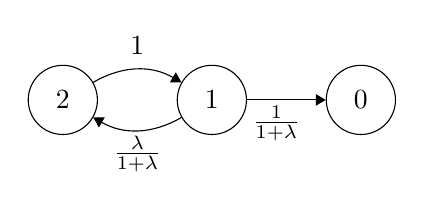
\begin{tikzpicture}[start chain = going right,
   -Triangle, every loop/.append style = {-Triangle}]
   \node[state, on chain]  (2) {2};
   \node[state, on chain]  (1) {1};
   \node[state, on chain]  (0) {0};
   
   % TODO: Need to add labels
   \draw (2) edge[bend left] node[yshift=3mm]{$1$} (1);
   \draw (1) edge[bend left] node[yshift=-3mm]{$\frac{\lambda}{1 + \lambda}$}(2);
   \draw (1) edge[left] node[xshift=3mm, yshift=-3mm]{$\frac{1}{1 + \lambda}$} (0);
   
\end{tikzpicture}
    \caption{Embedded discrete Markov chain for two node contact process}
    \label{fig:discrete_mc_two_contact}
\end{figure}

Let $T_\lambda$ be the time in which we hit $(0,0)$.
Denote the wait time while in node $(1,1)$ is exponentially distributed random variable $S$ with parameter $- q_{(1,1)} = 2$ and similarly the wait time while in node $(1,0)$ or $(0,1)$ is exponentially distributed with parameter $- q_{(1,0)} = 1 + \lambda$, denoted $T$.

Let $N$ be the number of times that the process waits at node $(1,0)$.
Note that this is equal to the number of times that the process waits at node $(1,1)$ since the transition $(1,1) \to (1,0)$ has probability 1.
$$
P(N = n) = \left(\frac{\lambda}{1 + \lambda} \right)^{n - 1} \frac{1}{1 + \lambda} \quad n = 1,2,\ldots
$$
with
\begin{align*}
    E[N] &= 1 + \lambda\\
    \Var(N) &= \frac{\lambda/(1 + \lambda)}{1/(1 + \lambda)^2} = \lambda (1 + \lambda)
\end{align*}

Let $S_1, S_2, \ldots$ be iid random variables with
$S_i \sim \exp(2)$ and independent of iid random variables $T_1, T_2, \ldots$ with  $T_i \sim \exp(1 + \lambda)$.
Denote $X_i \sim S_i + T_i$, Since the wait times are independent, then 
$$
E[X_i] = \frac{1}{2} + \frac{1}{1 + \lambda} = \frac{3 + \lambda}{2(1 + \lambda)}
$$

Now we can express $T_\lambda$ as a random sum
$$
T_\lambda = \sum_{i = 1}^N X_i
$$

\begin{theorem}
Let $X \sim \exp(\lambda)$ and $Y \sim \exp(\mu)$ be independent random variables with $T = \min(X,Y)$.
Then $T | X < Y \sim \exp(\lambda + \mu)$.
\end{theorem}

Using the theory of random sums \cite{Ross97}, TODO: Need to show that $X_i$ and $N$ are independent. we have that
$$
E[T_\lambda] = E\left[ \sum_{i = 1}^N X_i \right] = E[X_1] E[N] = \frac{3 + \lambda}{2(1 + \lambda)} \cdot (1 + \lambda) = \frac{3}{2} + \frac{\lambda}{2}
$$

Also, the variance of a random sum is defined as
\begin{align*}
    \Var\left( \sum_{i = 1}^N X_i \right) &= E[N]\Var(X) + (E[X])^2 \Var(N)\\
    &= (1 + \lambda) \frac{(1 + \lambda)^2 + 4}{4(1 + \lambda)^2} + \frac{(3 + \lambda)^2}{4 (1 + \lambda)^2} \lambda (1 + \lambda)^2\\
    &= \frac{\lambda^3 + 8 \lambda^2 + 17 \lambda + 14}{4(1 + \lambda)}\\
    &= \frac{\lambda^2 + 7 \lambda + 10}{4} + \frac{1}{1 + \lambda}
\end{align*}

\subsubsection{Limiting Distribution}

\begin{theorem} \label{thm:geom_sum}
Let $N$ be geometrically distributed with parameter $p$.
$P(N = n) = (1 - p)^{n - 1} p$ and $X_1,X_2,\ldots$ iid and independent of $N$ with each $X_i$ exponentially distributed with rate $\lambda$.
Then,
$$
\sum_{i = i}^N X_i \sim \exp(p \lambda)
$$
\end{theorem}

Thus,
\begin{align*}
    \sum_{i = 1}^N S_i &\sim \exp( \frac{2}{1 + \lambda})\\
    \sum_{i = 1}^N T_i &\sim \exp( 1 )
\end{align*}

Multiplying $T_\lambda$ by $\frac{2}{1 + \lambda}$ and using the scaling property of exponential random variables we have that
\begin{align*}
    \frac{2}{1 + \lambda}\sum_{i = 1}^N S_i &\sim \exp( 1 )\\
    \frac{2}{1 + \lambda}\sum_{i = 1}^N T_i &\sim \exp( \frac{2}{1 + \lambda})
\end{align*}
As $\lambda \to \infty$, then $T_\lambda \Rightarrow \exp(1)$

\subsection{Three node contact process}
Now we look at the three node contract process where all the nodes are connected.

Now let $N_1, N_2, N_3$ be the number of visits to states 1, 2, and 3, respectively.
Let $X_i^{(1)} \sim \exp(1 + 2\lambda)$ be iid random variables, $X_i^{(2)} \sim \exp(2 + 2\lambda)$ iid and $X_i^{(3)} \sim \exp(3)$ idd.
Not that these are not independent of each other, but for each $i$ each state is independent of the wait times at the state.

Then the discrete time Markov chain for this process can be expressed as
$$
P = \begin{blockarray}{cc|ccc}
    & 0 & 1 & 2 & 3\\
    \begin{block}{c(cccc)}
        0 & 0 & 0 & 0 & 0 \\
        \hline\\
        1 & \frac{1}{1 + 2\lambda} & 0 &
        \frac{2\lambda}{1 + 2\lambda} & 0\\
        2 & 0 & \frac{2}{2 + 2\lambda} & 0 & \frac{2}{2 + 2\lambda}\\
        3 & 0 & 0 & 1 & 0
    \end{block}
\end{blockarray}
$$
Since the discrete Markov chain \cite{grinstead2003}

\begin{figure}
    \centering
   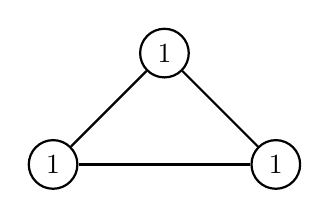
\begin{tikzpicture}[auto, node distance=2cm, every loop/.style={}, thick,main node/.style={circle,draw}]
   \node[main node]  (0) {1};
   \node[main node]  (1) [below left of=0]  {1};
   \node[main node]  (2) [below right of=0]  {1};
   
   \draw (0) edge [left] (1);
   \draw (0) edge [left] (2);
   \draw (1) edge [left] (2);
\end{tikzpicture}
    \caption{Three node contact process starting with initial state set as one.}
    \label{fig:three_node_contact_complete}
\end{figure}

\begin{figure}
    \centering
   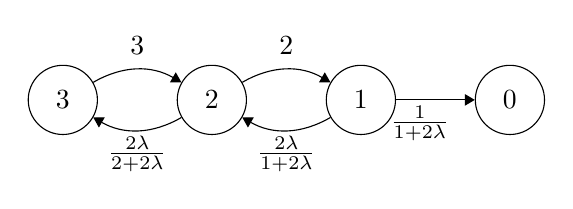
\begin{tikzpicture}[start chain = going right,
   -Triangle, every loop/.append style = {-Triangle}]
   \node[state, on chain]  (3) {3};
   \node[state, on chain]  (2) {2};
   \node[state, on chain]  (1) {1};
   \node[state, on chain]  (0) {0};
   
   \draw (3) edge[bend left] node[yshift=3mm]{$3$} (2);
   \draw (2) edge[bend left] node[yshift=-3mm]{$\frac{2 \lambda}{2 + 2 \lambda}$}(3);
   %
   \draw (2) edge[bend left] node[yshift=3mm]{$2$} (1);
   \draw (1) edge[bend left] node[yshift=-3mm]{$\frac{2\lambda}{1 + 2 \lambda}$}(2);
   %
   \draw (1) edge[left] node[xshift=3mm, yshift=-3mm]{$\frac{1}{1 + 2\lambda}$} (0);
   
\end{tikzpicture}
    \caption{Embedded discrete Markov chain for three node contact process}
    \label{fig:discrete_mc_three_contact}
\end{figure}

\subsubsection{Limiting Distribution}

\section{Finite contact process on 1D lattice}

The two node contact process on the lattice is identical to the complete graph.

\subsection{Three node contact process}

\begin{figure}
    \centering
   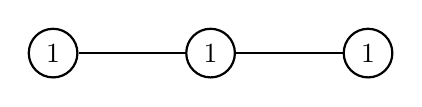
\begin{tikzpicture}[auto, node distance=2cm, every loop/.style={}, thick,main node/.style={circle,draw}]
   \node[main node]  (0) {1};
   \node[main node]  (1) [right of=0]  {1};
   \node[main node]  (2) [right of=1]  {1};
   
   \draw (0) edge [left] (1);
   \draw (1) edge [left] (2);
\end{tikzpicture}
    \caption{Three node contact process on 1D lattice}
    \label{fig:three_node_contact_lattice}
\end{figure}


\subsection{Voter Model}

\bibliographystyle{plainnat}
\bibliography{references}
\end{document}
